\documentclass{standalone}
\usepackage{tikz}
\usetikzlibrary{patterns, positioning}

\begin{document}
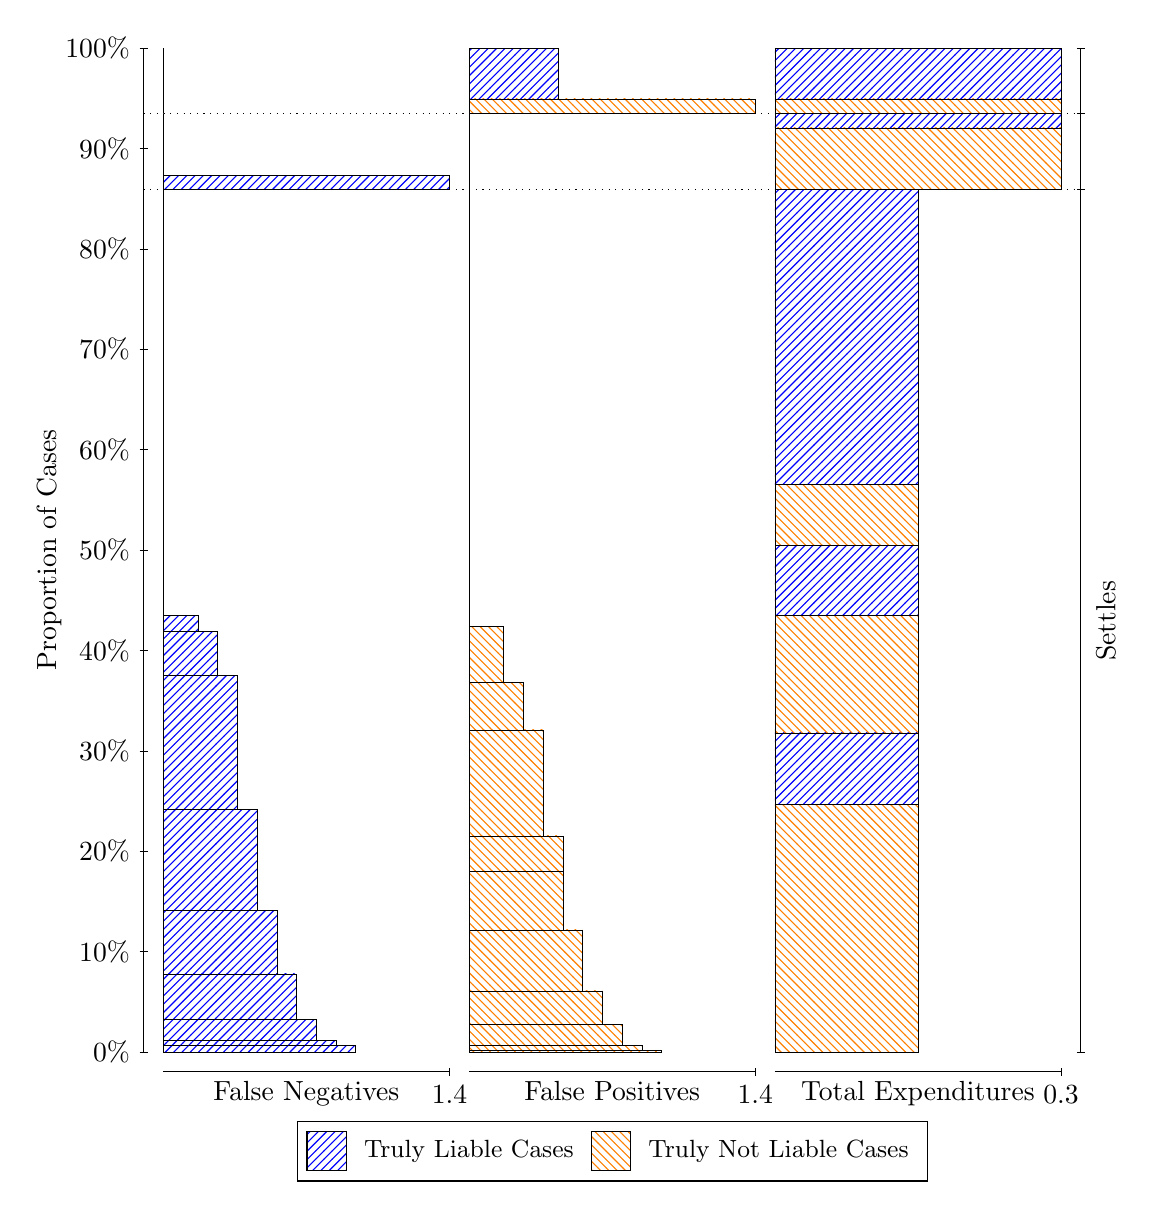
\begin{tikzpicture}
\draw[black, very thin] (1.5,1.75) -- (1.5,14.5);
\node[rotate=90, anchor=center] at (0.3, 8.125) {Proportion of Cases};
\draw[black, very thin] (1.45,1.75) -- (1.55,1.75);
\node[anchor=east] at (1.45, 1.75) {0\%};
\draw[black, very thin] (1.45,3.025) -- (1.55,3.025);
\node[anchor=east] at (1.45, 3.025) {10\%};
\draw[black, very thin] (1.45,4.3) -- (1.55,4.3);
\node[anchor=east] at (1.45, 4.3) {20\%};
\draw[black, very thin] (1.45,5.575) -- (1.55,5.575);
\node[anchor=east] at (1.45, 5.575) {30\%};
\draw[black, very thin] (1.45,6.85) -- (1.55,6.85);
\node[anchor=east] at (1.45, 6.85) {40\%};
\draw[black, very thin] (1.45,8.125) -- (1.55,8.125);
\node[anchor=east] at (1.45, 8.125) {50\%};
\draw[black, very thin] (1.45,9.4) -- (1.55,9.4);
\node[anchor=east] at (1.45, 9.4) {60\%};
\draw[black, very thin] (1.45,10.675) -- (1.55,10.675);
\node[anchor=east] at (1.45, 10.675) {70\%};
\draw[black, very thin] (1.45,11.95) -- (1.55,11.95);
\node[anchor=east] at (1.45, 11.95) {80\%};
\draw[black, very thin] (1.45,13.225) -- (1.55,13.225);
\node[anchor=east] at (1.45, 13.225) {90\%};
\draw[black, very thin] (1.45,14.5) -- (1.55,14.5);
\node[anchor=east] at (1.45, 14.5) {100\%};

\draw[black, very thin] (13.4,1.75) -- (13.4,14.5);
\draw[black, very thin] (13.35,1.75) -- (13.45,1.75);
\node[anchor=west] at (13.35, 1.75) {};
\draw[black, very thin] (13.35,12.701) -- (13.45,12.701);
\node[anchor=west] at (13.35, 12.701) {};
\draw[black, very thin] (13.35,13.67) -- (13.45,13.67);
\node[anchor=west] at (13.35, 13.67) {};
\draw[black, very thin] (13.35,14.5) -- (13.45,14.5);
\node[anchor=west] at (13.35, 14.5) {};

\draw[black, very thin, pattern color=blue, pattern=north east lines] (1.75,1.75) rectangle (4.1931,1.8308);
\draw[black, very thin, pattern color=blue, pattern=north east lines] (1.75,1.8308) rectangle (3.9425,1.9006);
\draw[black, very thin, pattern color=blue, pattern=north east lines] (1.75,1.9006) rectangle (3.692,2.164);
\draw[black, very thin, pattern color=blue, pattern=north east lines] (1.75,2.164) rectangle (3.4414,2.7422);
\draw[black, very thin, pattern color=blue, pattern=north east lines] (1.75,2.7422) rectangle (3.1908,3.5488);
\draw[black, very thin, pattern color=blue, pattern=north east lines] (1.75,3.5488) rectangle (2.9402,4.8322);
\draw[black, very thin, pattern color=blue, pattern=north east lines] (1.75,4.8322) rectangle (2.6897,6.5329);
\draw[black, very thin, pattern color=blue, pattern=north east lines] (1.75,6.5329) rectangle (2.4391,7.0865);
\draw[black, very thin, pattern color=blue, pattern=north east lines] (1.75,7.0865) rectangle (2.1885,7.2946);
\draw[black, very thin, pattern color=orange, pattern=north west lines] (1.75,7.2946) rectangle (1.75,12.701);
\draw[black, very thin, pattern color=blue, pattern=north east lines] (1.75,12.701) rectangle (5.3833,12.884);
\draw[black, very thin, pattern color=orange, pattern=north west lines] (1.75,12.884) rectangle (1.75,13.67);
\draw[black, very thin, pattern color=orange, pattern=north west lines] (1.75,13.67) rectangle (1.75,13.853);
\draw[black, very thin, pattern color=blue, pattern=north east lines] (1.75,13.853) rectangle (1.75,14.5);
\draw[black, very thin, pattern color=orange, pattern=north west lines] (5.6333,1.75) rectangle (8.0764,1.7691);
\draw[black, very thin, pattern color=orange, pattern=north west lines] (5.6333,1.7691) rectangle (7.8259,1.8325);
\draw[black, very thin, pattern color=orange, pattern=north west lines] (5.6333,1.8325) rectangle (7.5753,2.0998);
\draw[black, very thin, pattern color=orange, pattern=north west lines] (5.6333,2.0998) rectangle (7.3247,2.525);
\draw[black, very thin, pattern color=orange, pattern=north west lines] (5.6333,2.525) rectangle (7.0741,3.2999);
\draw[black, very thin, pattern color=orange, pattern=north west lines] (5.6333,3.2999) rectangle (6.8236,4.051);
\draw[black, very thin, pattern color=orange, pattern=north west lines] (5.6333,4.051) rectangle (6.8236,4.4951);
\draw[black, very thin, pattern color=orange, pattern=north west lines] (5.6333,4.4951) rectangle (6.573,5.8406);
\draw[black, very thin, pattern color=orange, pattern=north west lines] (5.6333,5.8406) rectangle (6.3224,6.4399);
\draw[black, very thin, pattern color=orange, pattern=north west lines] (5.6333,6.4399) rectangle (6.0718,7.1564);
\draw[black, very thin, pattern color=blue, pattern=north east lines] (5.6333,7.1564) rectangle (5.6333,12.701);
\draw[black, very thin, pattern color=orange, pattern=north west lines] (5.6333,12.701) rectangle (5.6333,13.487);
\draw[black, very thin, pattern color=blue, pattern=north east lines] (5.6333,13.487) rectangle (5.6333,13.67);
\draw[black, very thin, pattern color=orange, pattern=north west lines] (5.6333,13.67) rectangle (9.2667,13.853);
\draw[black, very thin, pattern color=blue, pattern=north east lines] (5.6333,13.853) rectangle (6.7609,14.5);
\draw[black, very thin, pattern color=orange, pattern=north west lines] (9.5167,1.75) rectangle (11.333,4.89);
\draw[black, very thin, pattern color=blue, pattern=north east lines] (9.5167,4.89) rectangle (11.333,5.8014);
\draw[black, very thin, pattern color=orange, pattern=north west lines] (9.5167,5.8014) rectangle (11.333,7.2928);
\draw[black, very thin, pattern color=blue, pattern=north east lines] (9.5167,7.2928) rectangle (11.333,8.1802);
\draw[black, very thin, pattern color=orange, pattern=north west lines] (9.5167,8.1802) rectangle (11.333,8.9553);
\draw[black, very thin, pattern color=blue, pattern=north east lines] (9.5167,8.9553) rectangle (11.333,12.701);
\draw[black, very thin, pattern color=orange, pattern=north west lines] (9.5167,12.701) rectangle (13.15,13.487);
\draw[black, very thin, pattern color=blue, pattern=north east lines] (9.5167,13.487) rectangle (13.15,13.67);
\draw[black, very thin, pattern color=orange, pattern=north west lines] (9.5167,13.67) rectangle (13.15,13.853);
\draw[black, very thin, pattern color=blue, pattern=north east lines] (9.5167,13.853) rectangle (13.15,14.5);
\draw[black, dotted] (1.5,12.701) -- (13.4,12.701);
\draw[black, dotted] (1.5,13.67) -- (13.4,13.67);
\draw[black, very thin] (1.75,1.5) -- (5.3833,1.5);
\node[anchor=north] at (3.5667, 1.5) {False Negatives};
\draw[black, very thin] (5.3833,1.45) -- (5.3833,1.55);
\node[anchor=north] at (5.3833, 1.45) {1.4};

\draw[black, very thin] (5.6333,1.5) -- (9.2667,1.5);
\node[anchor=north] at (7.45, 1.5) {False Positives};
\draw[black, very thin] (9.2667,1.45) -- (9.2667,1.55);
\node[anchor=north] at (9.2667, 1.45) {1.4};

\draw[black, very thin] (9.5167,1.5) -- (13.15,1.5);
\node[anchor=north] at (11.333, 1.5) {Total Expenditures};
\draw[black, very thin] (13.15,1.45) -- (13.15,1.55);
\node[anchor=north] at (13.15, 1.45) {0.3};

\node[black, centered, rotate=90] at (13.72, 7.2255) {Settles};



\draw (7.449999999999999,1.5) node[draw=none] (baseCoordinate) {};
\begin{scope}[align=center]
        \matrix[scale=0.5, draw=black, below=0.5cm of baseCoordinate, nodes={draw}, column sep=0.1cm]{
            \node[rectangle, draw, minimum width=0.5cm, minimum height=0.5cm, pattern=north east lines, pattern color=blue] {}; &
            \node[draw=none, font=\small] (B) {Truly Liable Cases}; &
            \node[rectangle, draw, minimum width=0.5cm, minimum height=0.5cm, pattern=north west lines, pattern color=orange] {}; &
            \node[draw=none, font=\small] (B) {Truly Not Liable Cases}; \\
            };
\end{scope}

\end{tikzpicture}
\end{document}